\documentclass[10pt]{article}
\usepackage{fullpage,enumitem,amsmath,amssymb,graphicx,subfig}
\usepackage{tikz}
\usepackage{array}
\usepackage{verbatim}

\begin{document}

\begin{center}
{\Large CS224N Winter 2016 Homework [3]}

\begin{tabular}{rl}
SUNet ID: & [jiajuns, xxx, xxx] \\
Name: & [Jiajun Sun, Sijun He, Mingxiang Chen] \\
\end{tabular}
\end{center}

By turning in this assignment, I agree by the Stanford honor code and declare
that all of this is my own work.

\section*{Problem 1: A window into NER}
\begin{enumerate}[label=(\alph*)]
\item
i.\\
Yesterday, price of Apple increased 6.56 percent.\\
Here apply can be interpreted as Apple the company or apple the fruit.\\
\\
Calvin Klein just released some nice designs for the winter season.\\
Here Calvin Klein can be interpreted as a name or a company.\\
\\
ii.\\
Words alone can have ambiguity, therefore adding features other than the word itself can help reduce ambiguity.\\
\\
iii.\\
First, the context of the word can help. The words around can imply the correct meaning of the center word.
Second, dependence structure within the window could shed light on the function of the center word in the sentences, which helps interpreting its entity.

\item
i.\\
$e^{(t)}$ has dimension of $1 \times (2w+1)D$\\
$W$ has dimension of $(2w+1)D \times H$\\
$U$ has dimension of $H \times C$\\
\\
ii.\\
$$
\begin{aligned}
& cost(ReLu) = \mathcal{O}(H) + \mathcal{O}((2w+1)D \times H)\\
& cost(softmax) = \mathcal{O}(H \times C) + \mathcal{O}(C)\\
& cost(CE) = \mathcal{O}(C)
\end{aligned}
$$
Given the sentences has length of $T$, the computation complexity is:
$$
\begin{aligned}
cost
& = T \times \mathcal{O}(\mathcal{O}(H) + \mathcal{O}((2w+1)D \times H) + \mathcal{O}(H \times C) + \mathcal{O}(C) + \mathcal{O}(C))\\
& \approx \mathcal{O}((2w+1)D \times H \times T)\\
& \approx \mathcal{O}(wDHT)
\end{aligned}
$$

\item
(code)

\item
i.\\
Entity level P/R/F1: 0.82/0.84/0.83\\
The confusion matrix shows that the model is very accurate in terms of classifying null class. Among all the entities,  ORG has the lowest precision and the lowest recall. The most commonly-made mistake by the model is misclassifying MISC entities as null.
\begin{table}[h]
	\centering
	\caption{confusion matrix}
	\begin{tabular}{|l|l|l|l|l|l|}
	\hline
	Acutal \textbackslash Predicted & PER     & ORG     & LOC     & MISC    & O        \\ \hline
	PER   & 2940.00 & 56.00   & 46.00   & 13.00   & 94.00    \\ \hline
	ORG   & 128.00  & 1676.00 & 92.00   & 63.00   & 133.00   \\ \hline
	LOC   & 54.00   & 119.00  & 1845.00 & 29.00   & 47.00    \\ \hline
	MISC  & 36.00   & 63.00   & 35.00   & 1018.00 & 116.00   \\ \hline
	O     & 37.00   & 42.00   & 12.00   & 31.00   & 42637.00 \\ \hline
	\end{tabular}
\end{table}

ii.\\
The first limitation is that the length of context is limited by the length of window size.
For example the \textbf{Test and County Cricket Board} does not get right label, because the length has exceeded the window size.\\
\\
The second limitation is that the model is too simplistic. The context is based solely on concatenating word vectors. The model can't decide which word in the context should it focus on. For example, \textbf{Grace Road} was not correctly classified in ``at Grace Road". The word ``at" is a very strong signal that the next word/phrases should be locations but the model fails to capture that. Currently the word ``at" has the same effect anywhere within the window. With a more sophisticated model like LSTM or GRU, we should be able to put emphasis on words that are more relevant to the entity.

\end{enumerate}
\clearpage
\section*{Problem 2:RNN for NER}
\begin{enumerate}[label=(\alph*)]
\item
i.\\
The number of RNN parameters:
$$
V \times D + H \times H + D \times H + H + H \times C + C
$$
The number of window-based model parameters:
$$
V \times D + (2w+1)D \times H + H + H \times C + C
$$
Therefore, RNN has $(H - 2wD)H$ more parameters than window-based model, assuming $H > 2wD$\\

ii.\\
Cost for one time step:
$$
\begin{aligned}
& cost(h) = \mathcal{O}(H \times H) + \mathcal{O}(D \times H) + \mathcal{O}(H)\\
& cost(softmax) = \mathcal{O}(H \times C) + \mathcal{O}(C)\\
& cost(CE) = \mathcal{O}(C)
\end{aligned}
$$
Adding them up:
$$
\mathcal{O}(H \times H) + \mathcal{O}(D \times H) + \mathcal{O}(H) + \mathcal{O}(H \times C) + \mathcal{O}(C) + \mathcal{O}(C) \approx \mathcal{O}(H \times H + D \times H)
$$
Therefore the total cost for sentence of length $T$:
$$
cost =  \mathcal{O}((H \times H + D \times H)T)
$$

\item
i.\\
The problem with cross entropy loss is that is maximize the softmax probability of the correct label instead of just classify the labels correctly. Consider a 2 token batch with 2 class, the labels are
$$y^{1} = [1, 0] \ \  y^{2} = [0, 1]$$
\textbf{Case 1}: $\hat{y}^{1} = [0.6, 0.4] \ \ \hat{y}^{2} = [0.4, 0.6]$. \\
The model gets both labels correct. $J = -2\text{log} \ 0.6 = 0.44$\par
\textbf{Case 2}: $\hat{y}^{1} = [0.99, 0.01] \ \ \hat{y}^{2} = [0.51, 0.49]$.\\
The model gets only 1 label correct. $J = -\text{log} \ 0.99 -\text{log} \ 0.49 = 0.31$\par
While case 2 has a smaller cross entropy loss, it only correctly classified one label and has a smaller $F_1$ score.\\

ii.\\
1. The $F_1$ score cannot be broken into token-level or batch-level terms and thus is impossible to do mini-batch optimization.
It requires looking through the entire training set, which is unrealistic in terms of memory. \\
2. There's no gradient of $F_1$ w.r.t. the parameters.
Optimizing $F_1$ will be ver hard since we need to reply on some variant of gradient descent for optimization.\\

\item
(code)

\item
The padded 0-vectors are at the end of the sentence.
When the model unroll to the padded 0-vectors, it will make predictions based solely on the past memory (current word input is all zeros).
Regardless of what the model predicts, it will add to the loss function.
Since the loss of these tokens (padded vectors) are not zero, it will produce a gradient and affect the batch gradient.
With masking, we neglect the loss terms of the padded 0-vectors. They no longer have any effect on the loss and thus no effect on the gradient.\\

\item
(code)

\item
Entity level P/R/F1: 0.84/0.86/0.85\\
The confusion matrix shows that the model is very accurate in terms of classifying null class. Among all the entities,  ORG has the lowest precision and MISC has the lowest recall.
\begin{table}[h]
	\centering
	\caption{confusion matrix}
	\begin{tabular}{|l|l|l|l|l|l|}
	\hline
	Acutal \textbackslash Predicted & PER     & ORG     & LOC     & MISC    & O        \\ \hline
	PER   & 2958.00 & 30.00   & 83.00   & 16.00   & 62.00    \\ \hline
	ORG   & 113.00  & 1676.00 & 108.00   & 88.00   & 107.00   \\ \hline
	LOC   & 32.00   & 70.00  & 1946.00 & 19.00   & 27.00    \\ \hline
	MISC  & 32.00   & 36.00   & 64.00   & 1042.00 & 94.00   \\ \hline
	O     & 37.00   & 46.00   & 35.00   & 38.00   & 42603.00 \\ \hline
	\end{tabular}
\end{table}

\item
The first limitation is signals in hidden layer dissipates in long range. For example, the model predicted ``Duran" as MISC instead of PER in ``Panamanian boxing legend Roberto "Hands of Stone" Duran climbs into..." Duran is a PER and it is strongly indicated by "boxing legend", however for RNN the signal fades too much when reaching ``Duran". Instead, the model predicted ``Hands" and ``Stone" as PER, possibly due to the strong signal. By the time the model unrolls to ``Duran", the signal in hidden layer has already dissipated and masked by the mixed signal from ``Hands" and ``Stone". \par
\vspace{5mm}
The second limitation is the RNN is one-directional and only uses the words before the target word to predict the entity. For example, the model predicted ``Washington" in ``The 11th-seeded Washington fell short of reprising his Wimbledon miracle comeback..." as a LOC instead of a PER, which makes sense when you only look at the words before ``Washington". But if the model can unroll bi-directionally and take into account the words after the target word like ``fell short of" or ``his", it will have done a better job.
\end{enumerate}
\clearpage
\section*{Problem 3:Grooving with GRUs}
\begin{enumerate}[label=(\alph*)]
\item
i.\\
$\boxed{U_h = 1, W_h = 1 \text{ and } b_h = 0}$\\
To replicate the behavior, the model always needs to preserve the memory ($W_h = 1$) to not forget the state of 1. It also need to always take new input ($W_x = 1$) so that it can react to the new input of 1.\par
ii.\\
$\boxed{U_z = 0, W_z = 1, U_h = 1 \text{ and } W_h \text{ can be any value.}}$\\
Given $w_r = u_r = b_r = 0$, the reset gate $r_t$ will always be zero. $\tilde{h}_t$ will be solely dependent on input ($U_h = 1$) and have no memory, thus $W_h$ can be any number. The objective is then have the update gate perform as following
$$z_t = \begin{cases}
 0, & x_t = 0 \text{ and } h_{t-1} = 0\\
 0, & x_t = 1 \text{ and } h_{t-1} = 0\\
 1, & h_{t-1} = 1\\
\end{cases}$$
We can achieve the above update gate behavior when $U_z=0$ and $W_z = 1$.
\item
i.\\
It is impossible for RNN to have togging behavior.
$U_t$ has to be a positive number in order to let $h_t$ switch to $1$.
Therefore for the second time when $x = 1$ it is impossible to let $h_t$ switch back to $0$.\\

ii.\\
$\boxed{b_r = 1, U_z = -1, W_z = 1, U_h = 1 \text{ and }W_h = -1}$\\
When $x_t=0$ and $h_{t-1} = 0$, $z_t = 0$ and $\tilde{h_t} = 0$, thus the hidden state will always be $h_t = 0$.\\
When $x_t=1$ and $h_{t-1} = 0$, $z_t = 0$ but $\tilde{h_t} = 1$, thus the hidden state will switch to $h_t = 1$.\\
When $h_{t-1}=1$ and $x_t=0$, $z_t = 1$, thus hidden state $h_t = h_{t-1} = 1$.\\
When $x_t=1$ and $h_{t-1} = 1$, $z_t = 0$, thus hidden state $h_t = \tilde{h}_t = 0$.\\
\item
(code)

\item
(i). The RNN model experiences vanishing gradient. Gradient Clipping does not help because it is not a solution to vanishing gradient, but exploding gradient.\\ 
While the GRU model has noisy gradients but it is not exploding. The model had its gradient clipped a couple times when it suddenly shot up, but there's no evidence in the result showing that the gradient clipping helped.\\
(ii). GRU performs better, as it was able to reach a much smaller minima compared with RNN. The reason is that GRU does not experience vanishing gradient like RNN so the error at a time step can provide feedback to words many steps away in the back propagation process. 
 
\begin{figure}[ht]
\centering
    \subfloat{{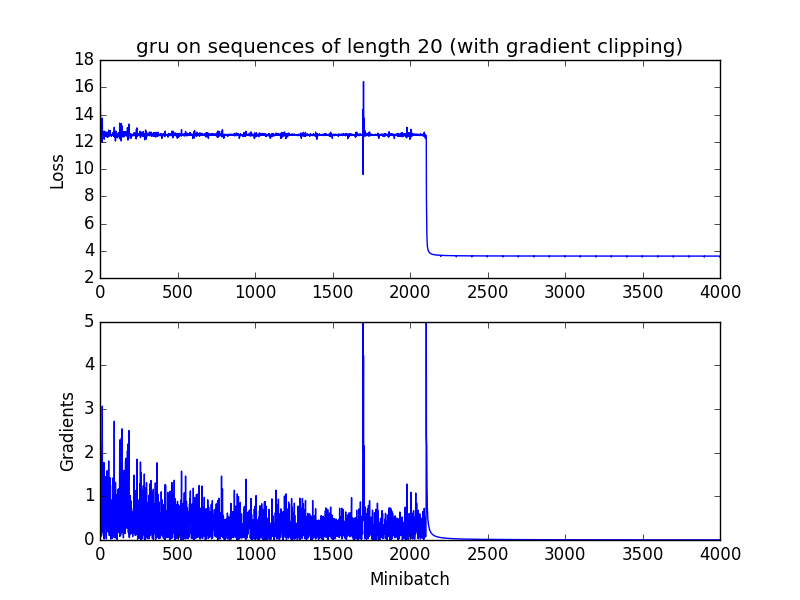
\includegraphics[scale=0.37]{q3-clip-gru.png} }}
    \qquad
    \subfloat{{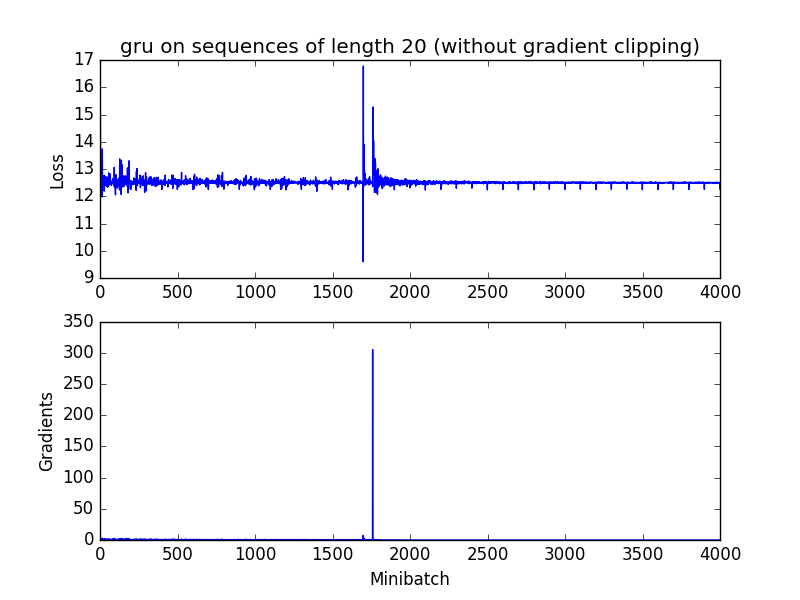
\includegraphics[scale=0.37]{q3-noclip-gru.png} }}
    \qquad
    \subfloat{{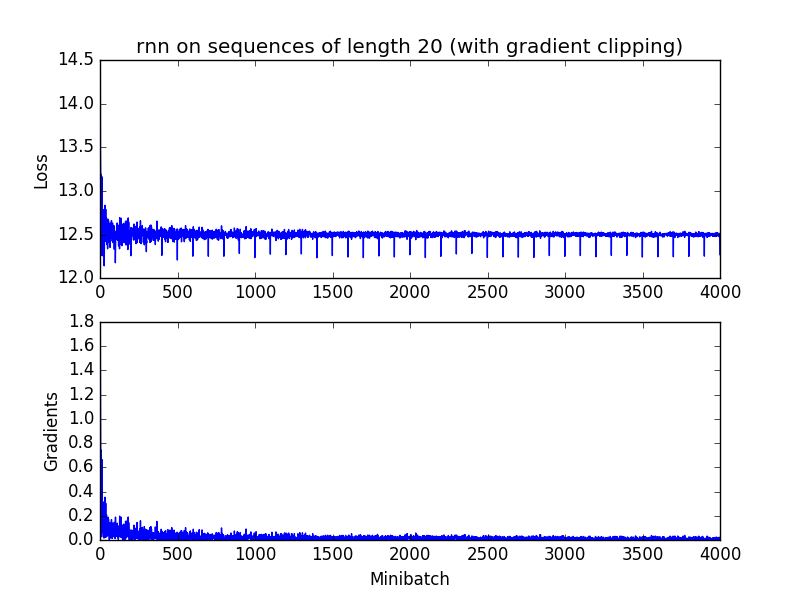
\includegraphics[scale=0.37]{q3-clip-rnn.png} }}
    \qquad        
    \subfloat{{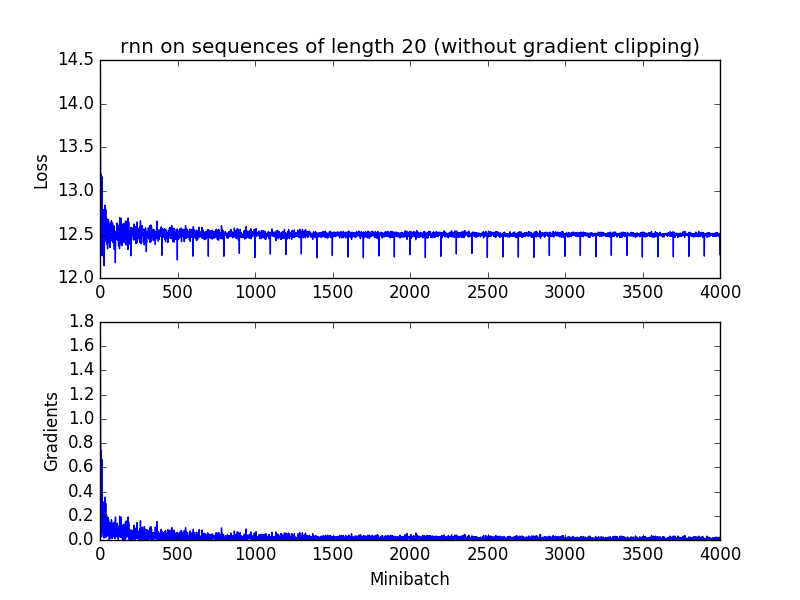
\includegraphics[scale=0.37]{q3-noclip-rnn.png} }}
\end{figure}


\item
Entity level P/R/F1: 0.86/0.86/0.86\\
\begin{table}[h]
	\centering
	\caption{confusion matrix}
	\begin{tabular}{|l|l|l|l|l|l|}
	\hline
	Acutal \textbackslash Predicted & PER     & ORG     & LOC     & MISC    & O        \\ \hline
	PER   & 2951.00 & 52.00   & 49.00   & 9.00   & 88.00    \\ \hline
	ORG   & 113.00  & 1718.00 & 58.00   & 77.00   & 126.00   \\ \hline
	LOC   & 32.00   & 79.00  & 1896.00 & 31.00   & 57.00    \\ \hline
	MISC  & 36.00   & 51.00   & 33.00   & 1046.00 & 102.00   \\ \hline
	O     & 31.00   & 63.00   & 20.00   & 27.00   & 42618.00 \\ \hline
	\end{tabular}
\end{table}

\end{enumerate}


\end{document}

